\documentclass{standalone}

\usepackage{tikz}
\usetikzlibrary{positioning}


\begin{document}

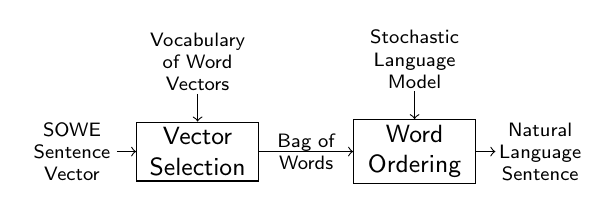
\begin{tikzpicture}[
	every node/.style={ text width=4em,
    					align=center,
                        font=\scriptsize\sffamily,
                        inner sep=1pt
                        },
	proc/.style= {draw,
    			  font=\small\sffamily,
                  inner sep = 2pt
    }
]
	\node (input) [inner sep=-4pt] {SOWE Sentence Vector};
    \node (selection) [proc, right = 0.7em of input]{Vector\\ Selection};
    \node (ordering) [proc, right = 3.4em of selection]{Word\\ Ordering};
	\node (vocab) [above = 1em of selection]{Vocabulary of Word Vectors};
    \node (lm) [above = 1em of ordering] {Stochastic Language Model};
    \node (output) [inner sep=-4pt, right=0.7em of ordering] {Natural Language Sentence};
    \draw[->] (input) -- (selection);
    \draw[->] (vocab) -- (selection);
    \draw[->] (selection) -- (ordering) node[midway] {Bag of Words};
    \draw[->] (lm) -- (ordering);
    \draw[->] (ordering) -- (output);
\end{tikzpicture}

\end{document}